\chapter{Design and Implementation}
\label{chapter-DesignAndImplementation}

This chapter discusses the design and implementation of the software that has
been developed as part of this thesis.

\section{Architecture}
\label{section-Architecture}

The workflow engine that has been developed as part of this thesis has been
designed and implemented as three loosely coupled components. The
\texttt{Workflow} component provides an object-oriented framework to define
workflows and an execution engine to execute them.
The \texttt{WorkflowDatabaseTiein} and \texttt{WorkflowEventLogTiein}
components tie the \texttt{Database} and \texttt{EventLog} components from the
eZ~Components library into the main \texttt{Workflow} component for persistence
and monitoring, respectively.

A workflow can be defined programmatically by creating and connecting objects
(see Section~\ref{section-Example}) that represent control flow constructs.
The classes for these objects are provided by the \emph{Workflow Definition API}
(see Appendix~\ref{chapter-API} for a reference). This API also provides the
functionality to save workflow definitions (ie. object graphs) to and load
workflow definitions from a data storage. Two data storage backends have been
implemented, one for relational database systems and another for XML files.
Through the \emph{Workflow Execution API} the execution of a workflow
definition can be started (and resumed). Figure \ref{figure-architecture}
shows the conceptual architecture for the workflow engine.

\clearpage

\begin{figure}[hbt]
\begin{center}
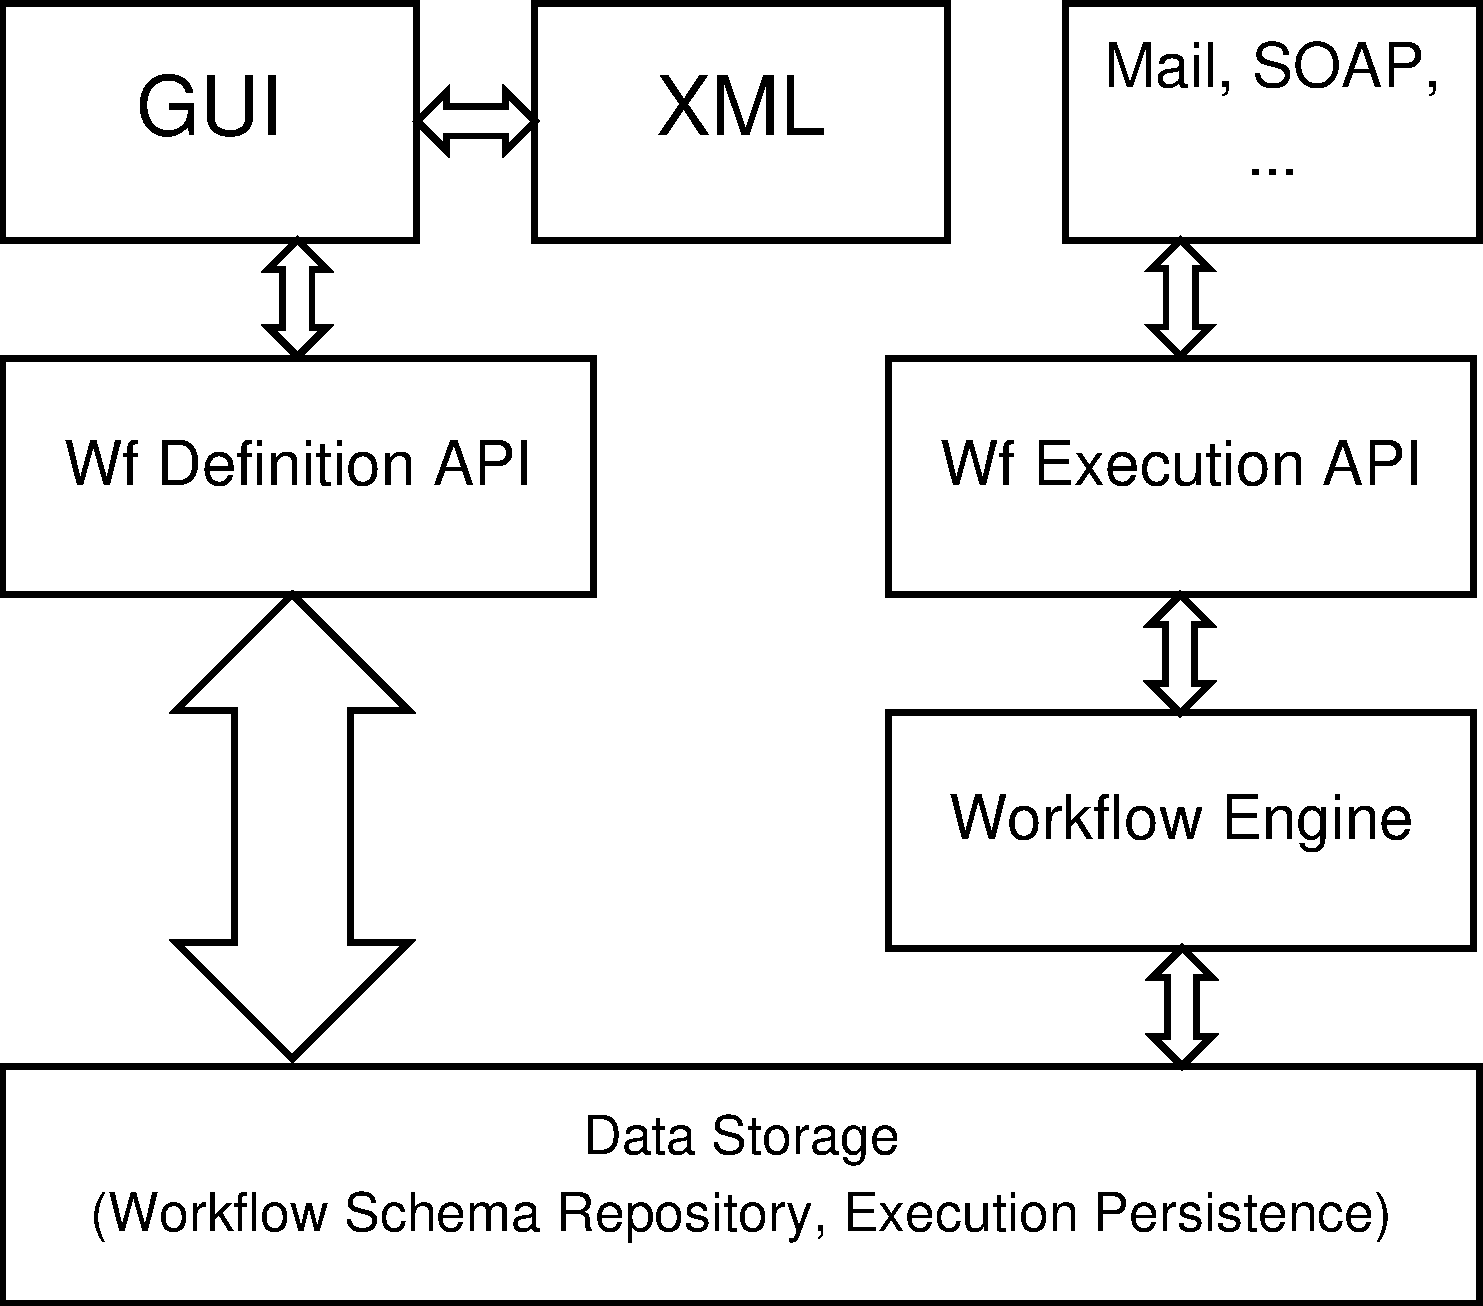
\includegraphics[width=10cm]{figures/architecture}\\[5mm]
\end{center}
\caption{Conceptual architecture for the workflow engine}
\label{figure-architecture}
\end{figure}

The idea that a workflow system should be comprised of loosely coupled
components is discussed, for instance, in \cite{DAM01,DG95,PM99}. Manolescu
states that

\begin{quote}
\emph{an object-oriented workflow architecture must \emph{provide abstractions}
that enable software developers to define and enact how the work flows through
the system} \cite{DAM01}.
\end{quote}

The component-based workflow architecture Micro-Workflow \emph{encapsulates
workflow features in separate components}. This architecture follows the
\emph{Microkernel} pattern which

\begin{quote}
\emph{applies to software systems that must be able to adapt to changing
system requirements. It separates a minimal functional core from extended
functionality and customer-specific parts. The microkernel also serves as a
socket for plugging in these extensions and coordinating their
collaboration} \cite{FB96}.
\end{quote}

The minimalistic core of Micro-Workflow is comprised of three components that
provide basic workflow functionality:

\begin{itemize}
\item The \emph{process component} implements an activity-based workflow model
      and provides the abstractions required to build workflows.
\item The \emph{execution component} implements the functionality to execute
      workflows.
\item The \emph{synchronization component} allows developers to define
      dependencies within the workflow domain.
\end{itemize}

On top of these core components other components, for instance for persistence
(suspending and resuming workflow execution), monitoring (status of running
workflows), history (history of executed workflows), and worklist management
(human-computer interface), can be implemented. Each of these components
\emph{encapsulates a design decision} and can be customized or replaced.

\section{Workflow Virtual Machine}
\label{section-WorkflowVirtualMachine}

This section proposes a so-called \emph{workflow virtual machine} as the
executing component of a component-based workflow architecture.

Given the fact that \emph{standardization efforts, e.g. XPDL \cite{WfMC05}
proposed by the WfMC, have essentially failed to gain universal acceptance}
\cite{WA04}, the \emph{problem of developing a [workflow system] that supports
changes in the [workflow description language]} needs to be addressed.

Fernandes et. al. propose to

\begin{quote}
\emph{split the [workflow system] into two layers: (1) a layer implementing
a \emph{Workflow Virtual Machine}, which is responsible for most of the
[workflow system] activities; and (2) a layer where the different [workflow
description languages] are handled, which is responsible for making the
mapping between each [workflow description language] and the Workflow Virtual
Machine} \cite{SF04}.
\end{quote}

A workflow virtual machine isolates the executing part of a workflow
management system, the \emph{backend}, from the parts that users interact
with, the \emph{frontend}. This isolation allows for the definition of a
\emph{backend language} to describe exactly the workflows that are supported
by the executer and its underlying workflow model. This backend language is
not the workflow description language users use to define their workflows.
They use \emph{frontend languages} that can be mapped to the system's
backend language.

\section{Graph-Oriented Programming}
\label{section-GraphOrientedProgramming}

The manual of JBoss jBPM \cite{JBOSS}, a platform for multiple process
languages supporting workflow, business process management, and process
orchestration, introduces \emph{Graph-Oriented Programming [as a] new
implementation technique that serves as a basis for all graph-based process
languages}.

Graph-Oriented Programming implements the \emph{graphical representation} and
the \emph{wait states} of a process language in an object-oriented programming
language. The former can be achieved by providing a framework of node classes.
Objects of these classes represent the nodes in the process graph, relations
between these objects represent the edges. Such an object graph can then be
traversed for execution. These executions need to be persistable, for instance
in a relational database, to support the wait states.

The aforementioned node classes implement the \emph{Command} design pattern
\cite{GoF94} and encapsulate an action and its parameters.

The executing part of the workflow engine is implemented in an
\texttt{Execution} class. An object of this class represents a workflow in
execution. The execution object has a reference to the current node. When the
execution of a workflow is started, a new execution object is created and the
current node is set to the workflow's start node. The \texttt{execute()}
method that is to be provided by the node classes is not only responsible for
executing the node's action, but also for propagating the execution:
\emph{a node can pass the execution that arrived in the node [to] one of its
leaving transitions to the next node}.

Like Fowler in \cite{MF05}, the authors of the JBoss jBPM manual acknowledge
the fact that \emph{current software development relies more and more on domain
specific languages}. They see Graph-Oriented Programming as a means to
implement domain specific languages \emph{that describe how graphs can be
defined and executed} on top of an object-oriented programming language.

In this context, a process language (like a workflow description language) is
\emph{nothing more than a set of \texttt{Node} implementations}. The semantics
of each node are defined by the implementation of the \texttt{execute()}
method in the respective node class. This language can be used as the backend
language of a Workflow Virtual Machine (see
Section~\ref{section-WorkflowVirtualMachine}). In this lanugage, the workflow
is represented as a graph of command objects. The workflow patterns (see
Section~\ref{section-WorkflowPatterns}) make up the requirements for and can
be mapped to the respective classes.

One of the advantages of using a domain specific language that Fowler gives in
\cite{MF05} regards the \emph{involvement of lay programmers: domain experts
who are not professional programmers but program in domain specific languages
as part of the development effort}. In essence this means that a software
system that provides a domain specific language can be customized and
extended without knowledge of the underlying programming language that was
used to implement it.

\section{Implementation Details}

The workflow engine maintains a set of activated nodes. At the beginning of
the execution, the workflow's start node is activated.

Listing~\ref{listing-ezcWorkflowExecution} shows the main execution loop of
the workflow virtual machine. As long as the workflow execution has not
explicitly ended (by reaching an \emph{End} node), the next activated node
is executed. After the node has been successfully executed it is removed from
the set of activated nodes. In a situation where the set of activated nodes
is not empty but none of the activated nodes can be completed (because they are
waiting for user input, for instance), the workflow execution is suspended.
When the set of activated nodes is empty, the execution of the workflow ends.

\begin{lstlisting}[language=PHP,float,caption={The workflow engine's main execution loop},label=listing-ezcWorkflowExecution]
<?php
abstract class ezcWorkflowExecution
{
    // ...

    protected function execute()
    {
        do
        {
            $executed = false;

            foreach ( $this->activatedNodes as $key => $node )
            {
                if ( !$this->hasEnded() )
                {
                    if ( $node->execute( $this ) )
                    {
                        unset( $this->activatedNodes[$key] );
                        $executed = true;
                    }
                }
            }
        }
        while ( !empty( $this->activatedNodes ) && $executed );

        if ( !$this->hasEnded() )
        {
            $this->suspend();
        }
    }

    // ...
}
?>
\end{lstlisting}

During its execution, a node can activate an arbitrary amount of its outgoing
nodes. \emph{Synchronization}, \emph{Synchronizing Merge}, and
\emph{Discriminator} nodes, for instance, need to be activated several times
before they can complete their execution.

Parallel threads of execution that are branched by the \emph{Parallel Split}
and \emph{Multi-Choice} (and merged by the \emph{Synchronization},
\emph{Synchronizing Merge}, and \emph{Discriminator}) workflow patterns are
executed serialized.

\clearpage
\section{Example}
\label{section-Example}

Listing~\ref{listing-Example.php} shows an example of PHP code that
programmatically creates an object graph for a workflow.

\begin{lstlisting}[language=PHP,float,caption={Creating an object graph using the \emph{Workflow Definition API}},label=listing-Example.php]
<?php
require_once 'Base/base.php';

function __autoload( $className )
{
    ezcBase::autoload( $className );
}

$workflow = new ezcWorkflow( 'Test' );

$input = new ezcWorkflowNodeInput(
  array(
    'choice' => 'boolean'
  )
);

$workflow->startNode->addOutNode( $input );

$branch = new ezcWorkflowNodeExclusiveChoice;
$branch->addInNode( $input );

$true  = new ezcWorkflowNodeAction( 'PrintTrue' );
$false = new ezcWorkflowNodeAction( 'PrintFalse' );

$branch->addConditionalOutNode(
  new ezcWorkflowConditionIsTrue(
    'choice'
  ),
  $true
);

$branch->addConditionalOutNode(
  new ezcWorkflowConditionIsFalse(
    'choice'
  ),
  $false
);

$merge = new ezcWorkflowNodeSimpleMerge;
$merge->addInNode( $true )
      ->addInNode( $false )
      ->addOutNode( $workflow->endNode );
?>
\end{lstlisting}

The workflow in this example consists of seven nodes:

\begin{enumerate}
\item A \emph{Start} node (line 10).
\item An \emph{Input} node (lines 13--17) that requests a boolean input
      variable.
\item An \emph{Exclusive Choice} node (line 21) that conditionally
      branches (lines 27--39) based upon the value of the previously
      supplied input variable.
\item An \emph{Action} node that has a \texttt{PrintTrue} service
      object attached to it (line 24).
\item An \emph{Action} node that has a \texttt{PrintFalse} service
      object attached to it (line 25).
\item A \emph{Simple Merge} node (lines 41--44).
\item An \emph{End} node (line 11).
\end{enumerate}

Listing~\ref{listing-XML} shows the object graph created by this PHP code
serialized to XML, Appendix~\ref{chapter-Tutorial} elaborates on this example
and explains it in detail.

\begin{lstlisting}[language=XML,firstnumber=1,stepnumber=100,float,caption={Workflow specification in XML markup},label=listing-XML]
<?xml version="1.0" encoding="UTF-8"?>

<workflow name="Test" version="1">
  <node id="1" type="Start">
    <outNode id="3"/>
  </node>

  <node id="2" type="End"/>

  <node id="3" type="Input">
    <variable name="choice" constraint="boolean"/>
    <outNode id="4"/>
  </node>

  <node id="4" type="ExclusiveChoice">
    <condition type="IsTrue" variable="choice">
      <outNode id="5"/>
    </condition>

    <condition type="IsFalse" variable="choice">
      <outNode id="6"/>
    </condition>
  </node>

  <node id="5" type="Action" serviceObjectClass="PrintTrue">
    <outNode id="7"/>
  </node>

  <node id="6" type="Action" serviceObjectClass="PrintFalse">
    <outNode id="7"/>
  </node>

  <node id="7" type="SimpleMerge">
    <outNode id="2"/>
  </node>
</workflow>
\end{lstlisting}

\clearpage
\section{Summary}

The core of the workflow engine that has been developed as part of this thesis
is a virtual machine that executes workflows represented through object graphs.
These object graphs can be created programmatically through the software
component's Workflow Definition API. Alternatively, a workflow definition can
be loaded from an XML file. Object graph and XML file are two different
representations of a workflow definition that uses the so-called backend
language of the workflow engine's core. Arbitrary frontend languages such as
the XML Process Definition Language (XPDL) \cite{WfMC05}, for instance, can be
mapped to the workflow engine's backend language.
